\documentclass[11pt,a4paper]{article}
\usepackage[margin=2.25cm]{geometry}
\usepackage{booktabs}
\usepackage{amsmath}
\usepackage{siunitx}
\usepackage{hyperref}
\usepackage{xcolor}
\usepackage{datetime}
\usepackage{adjustbox}
\newdateformat{monthyeardate}{\monthname[\THEMONTH] \THEYEAR}
\setlength{\tabcolsep}{4pt}

\title{Fine-tuning vs. Model Size vs. Parameter-Efficient Tuning (LoRA):\\
A Compact Experimental Report on Efficacy, Efficiency, and Reasoning Control}
\author{Alberto Rodero\thanks{Equal contribution} \and Pablo Lobato\footnotemark[1]}
\date{September 2025}

\sisetup{
  round-mode=places,
  round-precision=3,
  table-number-alignment=center
}

\begin{document}
\maketitle

\section{Introduction}
We evaluate the trade-offs between \textbf{full fine-tuning} (NoPeft), \textbf{LoRA}-based tuning with different ranks, and \textbf{base model size} using Qwen3-0.6B and Qwen3-1.7B on three task families: ARC (multiple-choice), OpenMath (numeric reasoning; lower is better), and SQuAD v2 (extractive QA). 
Additionally, we consider the model's \textbf{``reasoning'' mode} (a run-time behavior that may or may not be engaged depending on the generation configuration). In these runs, \emph{reasoning was not locked}, which can inject variance into both latency and accuracy. This report answers practical questions about whether, when, and how to fine-tune; how LoRA rank matters; how results compare to a larger base model; and how to set reasoning going forward.

\paragraph{Key questions.}
\begin{itemize}
  \item \textbf{Q1:} Is fine-tuning worth it in efficacy and efficiency?
  \item \textbf{Q2:} How does a fine-tuned 0.6B compare to a larger 1.7B base?
  \item \textbf{Q3:} If VRAM is abundant, is LoRA still worth using?
  \item \textbf{Q4:} Does LoRA rank materially affect outcomes?
  \item \textbf{Q5:} Partial vs.\ full tuning: LoRA vs.\ NoPeft?
  \item \textbf{Q6:} Cross-task transfer effects?
  \item \textbf{Q7:} If VRAM forces LoRA, is fine-tuning still worth it?
\end{itemize}

\section{Experimental Setup}
\paragraph{Models.} Qwen3-0.6B (fine-tuned on: ARC, OpenMath, SQuAD; with NoPeft and LoRA ranks $\{32,64,256,512,1024\}$), Qwen3-0.6B base, Qwen3-1.7B base.

\paragraph{Tasks \& metrics.} 
ARC: macro-F1 (higher is better). 
OpenMathInstruct-2: average absolute difference (lower is better). 
SQuAD v2: F1 (higher is better). 
We also record mean latency (seconds) per task.

\paragraph{Reasoning.} No explicit on/off control was enforced during these runs, so the model may have engaged/disengaged internal reasoning opportunistically. We treat this as a confound we will control in follow-up (Sec.~\ref{sec:reasoning}).

\section{Full Results Table}
\label{sec:fulltable}

\noindent\textit{Notes:} ``Math AbsDiff\,$\downarrow$'' is lower=better. Latencies are seconds. ``Train Dataset'' is the fine-tuning source (``\_base'' for none).

\begin{table}[htbp]
\centering
\caption{Full results across tasks. Lower is better for Math AbsDiff.\\
\footnotesize\emph{Notes:} Latency in seconds. ``Train DS'' is the fine-tuning source (``\_base'' = none).}
\label{tab:full}
\footnotesize
\begin{adjustbox}{max width=\textwidth}
\begin{tabular}{lrrrrrrl}
\toprule
{} &  ARC F1 & ARC Lat (s) & Math AbsDiff$\downarrow$ & Math Lat (s) & SQuAD F1 & SQuAD Lat (s) & Train DS \\
\midrule
Qwen3-0.6B-arc\_SFT\_None\_Lora1024 &  0.4921 & 0.1557 & 22,871 & 0.4374 &  8.59 & 0.1939 & arc \\
Qwen3-0.6B-arc\_SFT\_None\_Lora512  &  0.4861 & 0.1570 & 22,871 & 0.4312 &  8.59 & 0.1955 & arc \\
Qwen3-0.6B-arc\_SFT\_None\_Lora256  &  0.4921 & 0.1549 & 22,871 & 0.4191 &  8.59 & 0.1948 & arc \\
Qwen3-0.6B-arc\_SFT\_None\_Lora64   &  0.4937 & 0.1601 & 22,871 & 0.1811 &  8.09 & 0.1952 & arc \\
Qwen3-0.6B-arc\_SFT\_None\_Lora32   &  0.4880 & 0.1595 & 22,871 & 0.4439 &  8.59 & 0.1958 & arc \\
Qwen3-0.6B-arc\_SFT\_NoPeft\_NoQuant & 0.4905 & 0.0803 & 23,108 & 0.2137 & 18.89 & 0.2003 & arc \\
Qwen3-0.6B-openmath\_SFT\_None\_Lora1024 & 0.4990 & 0.9257 & 23,919 & 1.5384 &  8.48 & 0.2091 & openmath \\
Qwen3-0.6B-openmath\_SFT\_None\_Lora256  & 0.5031 & 0.8982 & 23,655 & 1.5016 &  8.48 & 0.1934 & openmath \\
Qwen3-0.6B-openmath\_SFT\_None\_Lora32   & 0.5095 & 0.8702 & 23,919 & 1.5776 &  8.48 & 0.1963 & openmath \\
Qwen3-0.6B-openmath\_SFT\_NoPeft\_NoQuant & 0.5171 & 0.0605 & 16,540 & 0.0482 &  7.40 & 0.2439 & openmath \\
Qwen3-0.6B-squad\_SFT\_None\_Lora1024 & 0.5024 & 0.3178 & 23,647 & 2.1285 &  9.59 & 0.1951 & squad \\
Qwen3-0.6B-squad\_SFT\_None\_Lora256  & 0.5024 & 0.3116 & 23,647 & 2.0291 &  9.59 & 0.1908 & squad \\
Qwen3-0.6B-squad\_SFT\_None\_Lora32   & 0.5024 & 0.3095 & 23,523 & 1.9676 &  9.59 & 0.1950 & squad \\
Qwen3-0.6B-squad\_SFT\_NoPeft\_NoQuant & 0.4542 & 0.1903 & 22,997 & 0.2203 & 27.95 & 0.2202 & squad \\
Qwen3-0.6B\_base                     & 0.4932 & 1.1397 & 24,834 & 6.0139 & 10.07 & 0.2274 & \_base \\
Qwen3-1.7B\_base                     & 0.7986 & 3.4025 &    742 &12.5197 & 30.36 & 0.2837 & \_base \\
\bottomrule
\end{tabular}
\end{adjustbox}
\end{table}

\section{Results by Question \& Interpretation}

\subsection*{\textbf{Q1. Is fine-tuning worth it (efficacy \& efficiency)?}}
\textbf{Yes, when aligned to the target task, fine-tuning yields large quality gains and often lower latency.} 
\begin{itemize}
  \item \textbf{OpenMath SFT (NoPeft)}: Math abs diff improves by \textbf{33.4\%} vs 0.6B\_base; ARC macro-F1 rises \textbf{+4.8\%}; SQuAD F1 drops \textbf{--26.5\%}. Latency massively drops on ARC (\textbf{--94.7\%}) and Math (\textbf{--99.2\%}), small increase on SQuAD (\textbf{+7.3\%}).
  \item \textbf{SQuAD SFT (NoPeft)}: SQuAD F1 jumps \textbf{+177.6\%}; ARC macro-F1 dips \textbf{--7.9\%}; Math improves mildly (\textbf{+7.4\%} abs-diff reduction). Latency generally improves (ARC \textbf{--83.3\%}, Math \textbf{--96.3\%}, SQuAD \textbf{--3.2\%}).
\end{itemize}
\textit{Why?} Full-task alignment amplifies the relevant capabilities and stabilizes decoding behavior; our pipeline also appears to run tuned checkpoints more efficiently.

\subsection*{\textbf{Q2. Fine-tuned 0.6B vs.\ larger 1.7B base?}}
\textbf{The 1.7B base dominates on quality but is slower.} 
ARC macro-F1 +61.9\%, Math abs diff $\sim$97\% better, and SQuAD F1 +201.5\% vs 0.6B\_base. Latency worsens markedly (ARC +198.5\%, Math +108.2\%, SQuAD +24.8\%). 
\textbf{If latency/throughput matters, 0.6B + targeted SFT is the speed/price sweet spot.}

\subsection*{\textbf{Q3. If VRAM is not a problem, should we still use LoRA?}}
\textbf{No. Prefer full fine-tuning.} In these runs, \textbf{NoPeft is both more accurate and often faster} than LoRA (Table~\ref{tab:lora_vs_nopeft}). The only place where NoPeft is slightly slower is SQuAD (+0.029\,s), but it delivers a \textbf{+18.36} absolute F1 jump over the best LoRA.

\begin{table}[htbp]
\centering
\caption{Best LoRA vs.\ NoPeft by task.}
\label{tab:lora_vs_nopeft}
\footnotesize
\begin{adjustbox}{max width=\textwidth}
\begin{tabular}{llrrrrl}
\toprule
Task & Best LoRA model & Best LoRA score & Best LoRA lat (s) & NoPeft model & NoPeft score & NoPeft lat (s) \\
\midrule
ARC & Qwen3-0.6B-arc\_SFT\_None\_Lora64 & 0.4937 & 0.1601 & Qwen3-0.6B-arc\_SFT\_NoPeft\_NoQuant & 0.4905 & 0.0803 \\
OpenMath (abs diff $\downarrow$) & Qwen3-0.6B-openmath\_SFT\_None\_Lora256 & 23{,}655 & 1.5016 & Qwen3-0.6B-openmath\_SFT\_NoPeft\_NoQuant & 16{,}540 & 0.0482 \\
SQuAD & Qwen3-0.6B-squad\_SFT\_None\_Lora1024 & 9.59 & 0.1951 & Qwen3-0.6B-squad\_SFT\_NoPeft\_NoQuant & 27.95 & 0.2202 \\
\bottomrule
\end{tabular}
\end{adjustbox}
\end{table}

\subsection*{\textbf{Q4. Does LoRA rank matter?}}
\textbf{Little to no monotonic benefit from increasing rank.} 
Correlation between rank and score (LoRA-only subsets): \textbf{ARC F1:} $\rho\!=\!0.021$; \textbf{OpenMath abs diff:} $\rho\!=\!0.301$ (higher rank slightly worse); \textbf{SQuAD F1:} constant across ranks (no signal). Rank vs.\ latency has weak-to-moderate correlations (e.g., ARC $\rho\!=\!-0.646$ suggests slightly lower latency at higher ranks, but absolute differences are tiny).
\begin{table}[h!]
\centering
\caption{Correlation between LoRA rank and performance/latency (LoRA-only).}
\label{tab:correlations}
{\small
\begin{tabular}{lrr}
\toprule
Task & Corr(rank, score) & Corr(rank, latency) \\
\midrule
ARC (F1) & 0.021 & -0.646 \\
OpenMath (AbsDiff$\downarrow$) & 0.301 & -0.233 \\
SQuAD (F1) & N/A & 0.321 \\
\bottomrule
\end{tabular}
}
\end{table}

\textit{Why might rank not matter much?} With limited data or strongly structured tasks, the low-rank subspace often captures the critical adaptations; beyond a point, extra capacity (higher rank) faces diminishing returns and optimization noise. Also, our decoding and “reasoning” variability likely masks small rank effects.

\subsection*{\textbf{Q5. LoRA (partial) vs.\ NoPeft (full) training?}}
\textbf{Full fine-tuning wins decisively.} 
OpenMath: NoPeft improves error by \textbf{7{,}115} absolute over best LoRA and is \textbf{$\sim$1.45\,s} faster. 
SQuAD: NoPeft improves F1 by \textbf{+18.36} with only \textbf{+0.029\,s} latency penalty. 
ARC: NoPeft is \textbf{$\sim$2$\times$ faster} than best LoRA, with essentially tied F1.

\subsection*{\textbf{Q6. Cross-task transfer?}}
\textbf{Positive and negative transfer exist; pick your anchors carefully.}
\begin{itemize}
  \item \textbf{OpenMath~SFT (NoPeft)} $\rightarrow$ ARC: \textbf{+4.8\%} (helpful), \; SQuAD: \textbf{--26.5\%} (harmful).
  \item \textbf{SQuAD~SFT (NoPeft)} $\rightarrow$ ARC: \textbf{--7.9\%} (harmful), \; Math: \textbf{+7.4\%} (helpful).
  \item \textbf{ARC~SFT (NoPeft)} $\rightarrow$ SQuAD: \textbf{+87.6\%} (surprisingly helpful), \; Math: \textbf{+7.0\%}; ARC itself: \textbf{--0.5\%} (negligible).
\end{itemize}
\textit{Interpretation.} Extractive QA and numeric reasoning compete for capacity in different ways; tuning to one can suppress behaviors useful to the other. ARC SFT (full) seems to improve general reading/selection that transfers to SQuAD, while OpenMath SFT strengthens procedural reasoning that can conflict with extractive behavior.

\subsection*{\textbf{Q7. If VRAM forces LoRA, is it still worth it?}}
\textbf{Yes, but temper expectations.} 
OpenMath LoRA-256 reduces error by \textbf{4.8\%} vs 0.6B\_base (useful), but SQuAD LoRA variants lose \textbf{$\sim$4.8\%} F1 vs 0.6B\_base, and ARC LoRA gains are marginal (\textbf{+0.1\%}). 
\textbf{Recommendation:} When constrained, \textbf{LoRA~$\approx$~256} is a good default; otherwise prefer NoPeft.

\section{Limitations}
\textbf{Reasoning mode was uncontrolled} (confound). 
\textbf{Single-seed/shot artifacts} may exist. 
\textbf{Latency} reflects this pipeline/hardware; other stacks may differ.
No calibration/temperature sweeps are reported here.

\section{Conclusions \& Takeaways}
\begin{itemize}
  \item \textbf{(1) Full fine-tuning beats LoRA on both accuracy and, in these runs, speed.}
  \item \textbf{(2) A larger base model is best on accuracy but slower; 0.6B+SFT is the speed/value sweet spot.}
  \item \textbf{(3) LoRA rank has weak, non-monotonic effects; use $\sim$256 by default when constrained.}
\end{itemize}
\begin{figure}
    \centering
    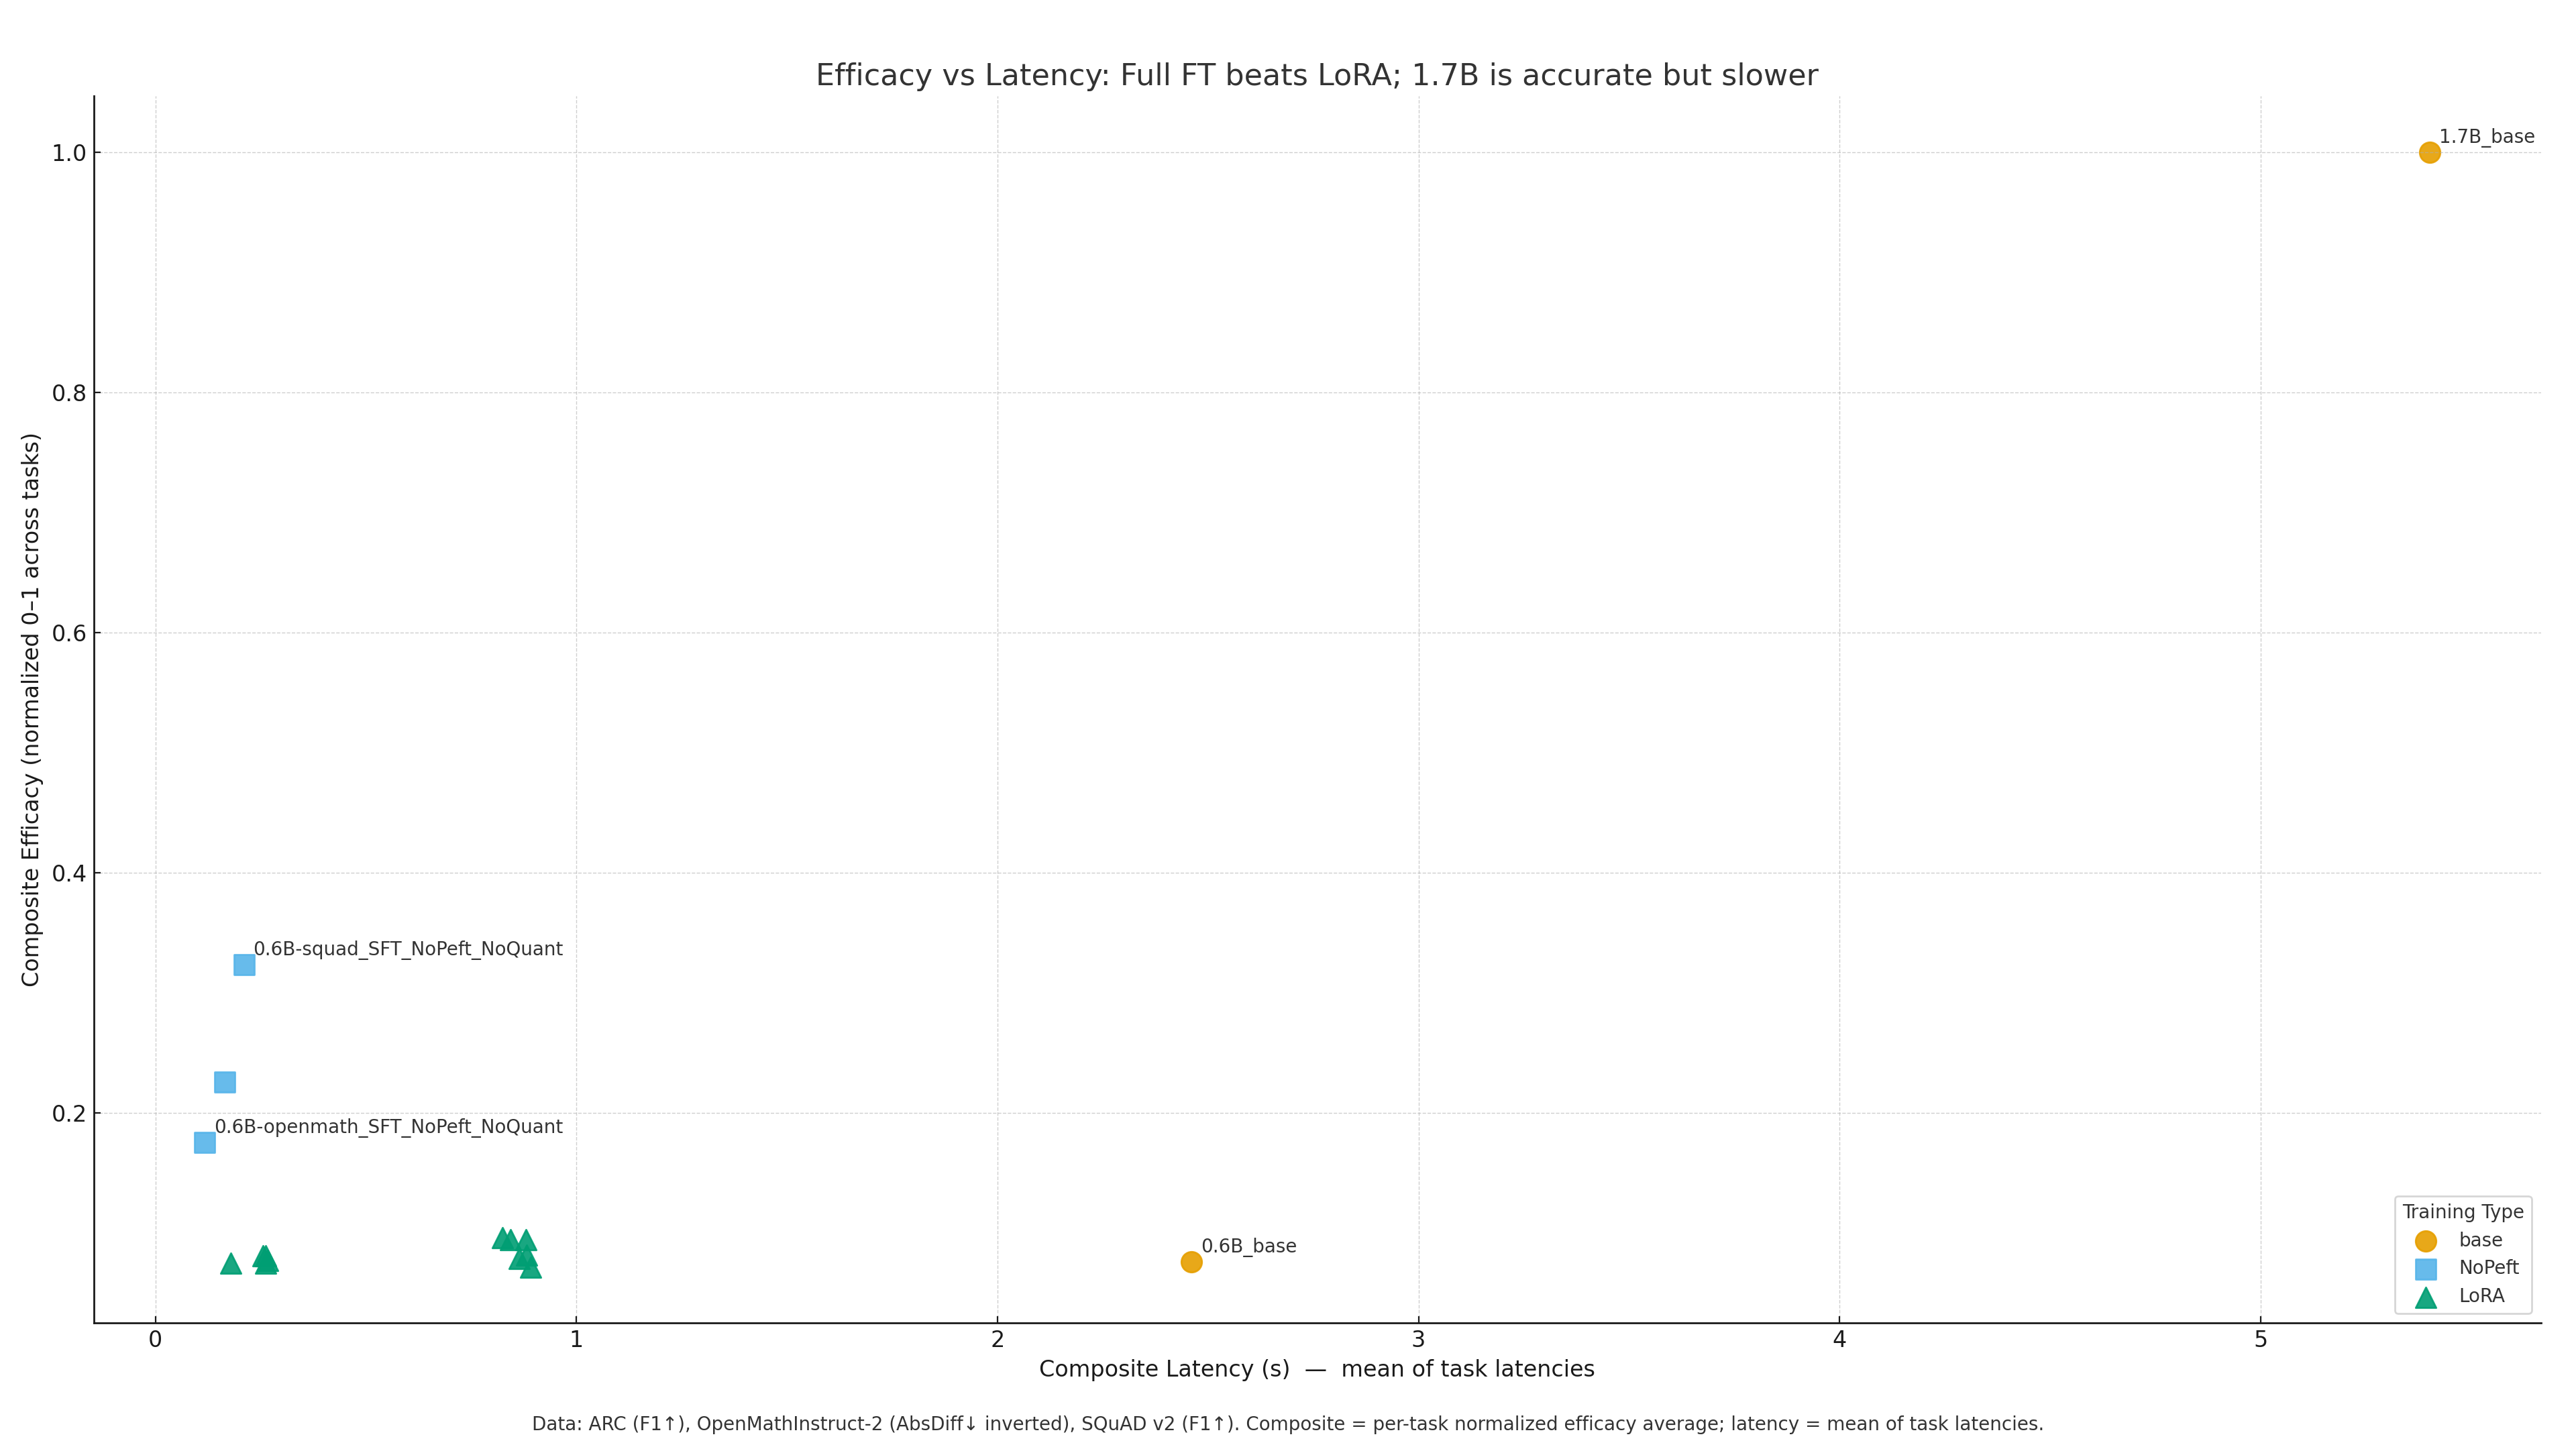
\includegraphics[width=1\linewidth]{01_Finetuning_ModelSize_LoraR.png}
    \caption{Efficacy vs Latency}
    \label{fig:placeholder}
\end{figure}

\end{document}
